\documentclass[xcolor=dvipsnames]{beamer}
\usecolortheme[named=Orange]{structure}
\usetheme{Warsaw}

\usepackage{multicol}
\usepackage{caption} % podpisy pod obrazkami
\usepackage[export]{adjustbox} % ramki dla obrazków
\usepackage{pgfplots} % wykresy
\usepackage{amsmath} % wzory funkcji
\usepackage{amsfonts}
\usepackage{xcolor,colortbl}
\usepackage{tex/slashbox} % łamana linia w górnym lewym rogu tabeli (podzielenie komórki na dwie)

\usepackage{polski}
\usepackage[utf8x]{inputenc}

% nowa komenda: defeq jako znaczek = z napisem def na górze
\newcommand\defeq{\mathrel{\overset{\makebox[0pt]{\mbox{\normalfont\tiny\sffamily def}}}{=}}}

% pisanie Rys. zamiast Rysunek pod obrazkami
\renewcommand{\figurename}{Rys.}

\setbeamerfont{caption}{series=\normalfont,size=\fontsize{7}{7}}

% numerowanie slajdów
\expandafter\def\expandafter\insertshorttitle\expandafter{%
  \insertshorttitle\hfill%
\insertframenumber\,/\,\inserttotalframenumber}

% slajdy z planem każdej sekcji
%\AtBeginSection[]
%{
%  \begin{frame}
%    \frametitle{Plan prezentacji}
%    \tableofcontents[currentsection]
%  \end{frame}
%}

% referencje
\usepackage[absolute,overlay]{textpos}
\newenvironment{reference}[2]{%
  \begin{textblock*}{\textwidth}(#1,#2)
\footnotesize\it\bgroup\color{red!50!black}}{\egroup\end{textblock*}}

\title[Obrona pracy dyplomowej]{Metody głębokiego uczenia w wybranych problemach klasyfikacji}
\subtitle[]{}
\author[J. Witkowski]{Jacek Witkowski}
\institute[Instytut Informatyki]{
  PW EiTI \\
  Instytut Informatyki \\
  promotor: mgr inż.~Rajmund Kożuszek
}
\date[Maj 2017]{30 maja 2017}

\begin{document}

% strona tytułowa
\begin{frame}[plain]
  \titlepage
\end{frame}

% plan prezentacji
\begin{frame}{Plan prezentacji}
  \tableofcontents
\end{frame}

\section{Wprowadzenie}
\subsection{Filtry splotowe}
\begin{frame}{Splot dyskretny}
    \begin{block}{Definicja}
        \begin{equation*}
            f\ast g[n]\defeq \sum\limits_{m=-\infty}^{\infty}f[m]g[n-m] = \sum\limits_{m=-\infty}^{\infty}f[n-m]g[m]
        \end{equation*}
        gdzie $f$ i $g$ to~ciągi splatane, a~zapis $f[n]$ to~zapis oznaczający $n$-ty wyraz ciągu $f$.
    \end{block}
    \begin{figure}
		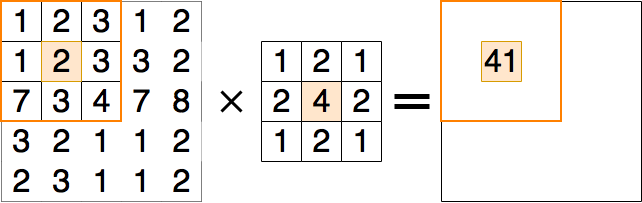
\includegraphics[width=\linewidth, keepaspectratio] {img/convolutional_filter.png}
	\end{figure}
\end{frame}
\begin{frame}{Filtr Gaussa}
    \begin{minipage}[t]{0.48\linewidth}
        Obraz wejściowy:
        \begin{figure}
            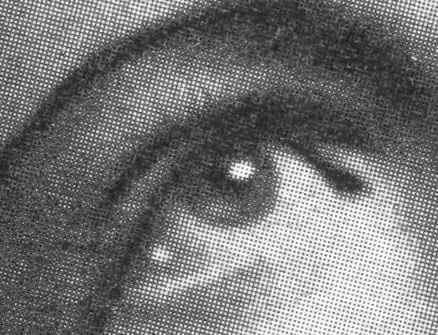
\includegraphics[width=\textwidth]{img/gauss-conv-real-input.jpg}
        \end{figure}
	\end{minipage}%
	\hfill
	\begin{minipage}[t]{0.48\linewidth}
        Obraz wyjściowy:
        \begin{figure}
            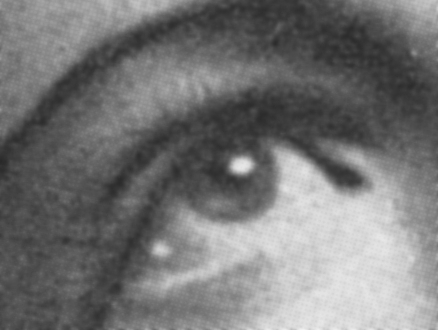
\includegraphics[width=\textwidth]{img/gauss-conv-real-output.jpg}
        \end{figure}
	\end{minipage}
\end{frame}
\subsection{Sieci splotowe}
\begin{frame}{Sieci splotowe}
    Splotowe sieci neuronowe:
    \begin{itemize}
        \item wykorzystują wiele filtrów splotowych,
        \item jądra filtrów splotowych są ustalane w procesie uczenia sieci,
        \item wynikami splotów są kolejne obrazy (tzw.~mapy cech),
        \item dokonują skalowania map cech w~celu redukcji rozmiaru przetwarzanych danych,
        \item w~końcowych etapach przetwarzania wykorzystywane są warstwy w~pełni połączone.
    \end{itemize}
\end{frame}
\begin{frame}{Faza I - Splot}
	\begin{figure}
		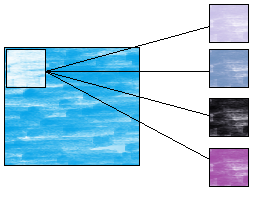
\includegraphics[width=\linewidth, height=0.7\textheight, keepaspectratio] {img/convolution.png}
	\end{figure}
\end{frame}
\begin{frame}{Faza II - Próbkowanie (\textit{ang.~subsampling})}
	\begin{minipage}[t]{0.6\linewidth}
		\begin{itemize}
			\item szybko rosnący rozmiar danych wyjściowych dla kolejnych warstw,
			\item zmniejszanie rozmiaru danych przez zmniejszanie obrazków,
			\item average pooling i max-pooling.
		\end{itemize}
	\end{minipage}%
	\hfill
	\begin{minipage}[t]{0.3\linewidth}
		\vfill
		\begin{figure}
			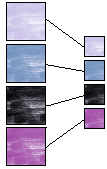
\includegraphics[width=\linewidth, height=0.7\textheight, keepaspectratio] {img/pooling.png}
		\end{figure}
	\end{minipage}
\end{frame}

\begin{frame}{Faza końcowa}
	\begin{figure}
		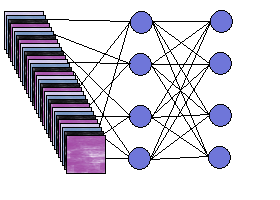
\includegraphics[width=\linewidth, height=0.7\textheight, keepaspectratio] {img/fully_connected_layer.png}
	\end{figure}
\end{frame}


\subsection{Zabiegi zwiększające jakość klasyfikacji}
\begin{frame}{Zwiększanie jakości klasyfikacji}
    \begin{minipage}[t]{0.48\linewidth}
        \begin{itemize}
            \item regularyzacja: zapobieganie przeuczeniu sieci (\textit{ang.~overfitting}),
            \item normalizacja (np.~lokalna normalizacja odpowiedzi).
        \end{itemize}
	\end{minipage}%
	\hfill
	\begin{minipage}[t]{0.48\linewidth}
        \begin{figure}
            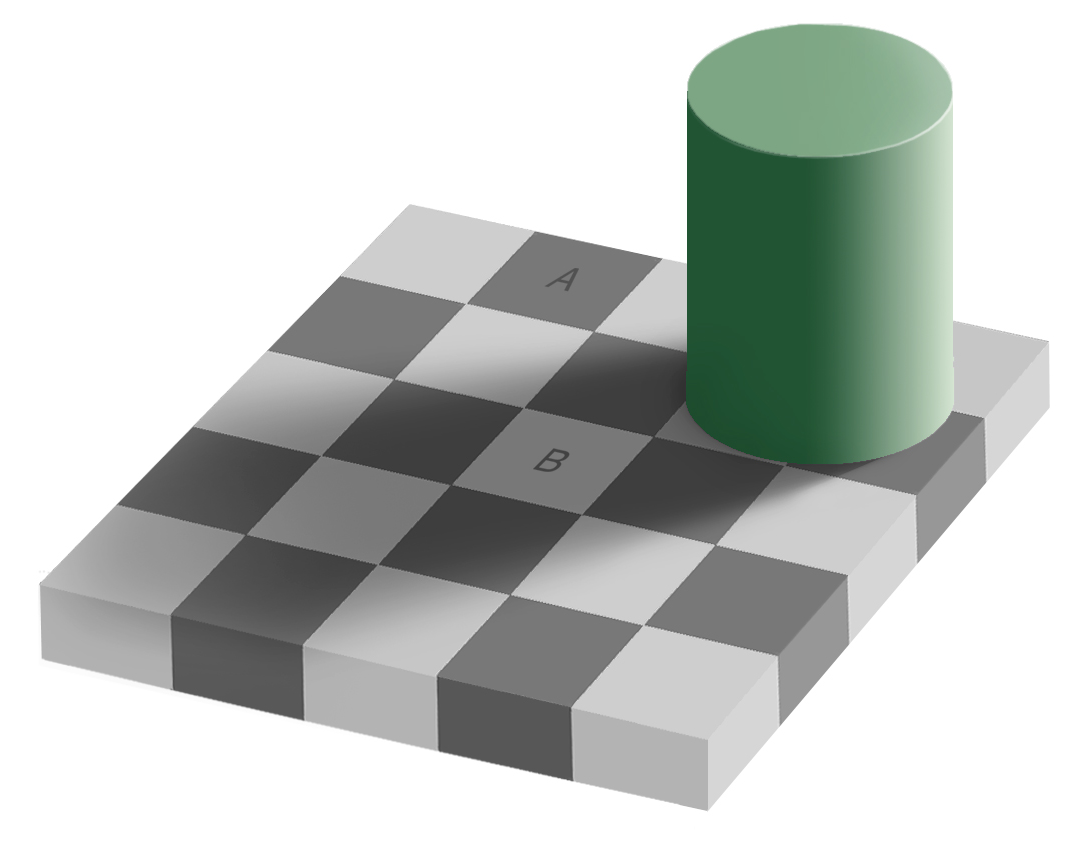
\includegraphics[width=\linewidth, height=0.7\textheight, keepaspectratio] {img/chess-illusion.png}
            \caption{Lokalna normalizacja odpowiedzi. \\
            Pola A i B mają ten sam kolor.}
        \end{figure}
	\end{minipage}
\end{frame}

\section{Badania}
\subsection{Cel badań}
\begin{frame}{Cel badań}
	\begin{itemize}
	    \item \textbf{Cel badań:} zbadanie wpływu regularyzacji L2 i lokalnej normalizacji odpowiedzi na~jakość
	    klasyfikacji.
	    \item \textbf{Jakość klasyfikacji:} dokładność, czyli stosunek poprawnie sklasyfikowanych przykładów
	           do~całkowitej liczby przykładów.
    \end{itemize}
\end{frame}
\subsection{Dobór wartości hiperparametrów}
\begin{frame}{Dobór wartości hiperparametrów}
    \begin{block}{Badane hiperparametry}
        \textbf{$\lambda$}~--~określa wpływ regularyzacji L2 (im~większa wartość, tym~większy wpływ)

        \vspace{2mm}
        \textbf{$\alpha$}~--~określa intensywność lokalnej normalizacji odpowiedzi (im~większa wartość,
        tym~większa intensywność).
    \end{block}
    \begin{block}{Metoda poszukiwań}
        \textbf{Przeszukiwanie kratowe} (\textit{ang.~grid search})~--~zbadanie wszystkich możliwych par parametrów
        $\lambda$ i~$\alpha$, gdzie badane wartości każdego z~parametrów należą do~pewnego skończonego dyskretnego
        zbioru
    \end{block}
\end{frame}
\subsection{Eksperymenty}
\begin{frame}{Architektura sieci}
    Warstwy badanych sieci:
    \begin{enumerate}
        \item Warstwa splotowa z 64 maskami 5x5x3,
        \item Warstwa skalująca typu max-pooling o rozmiarze 3x3x1 (przesunięcie: 2 piksele),
        \item Warstwa lokalnej normalizacji odpowiedzi,
        \item Warstwa splotowa z 64 maskami 5x5x64,
        \item Warstwa lokalnej normalizacji odpowiedzi,
        \item Warstwa skalująca typu max-pooling o rozmiarze 3x3x1 (przesunięcie: 2 piksele),
        \item Warstwa w~pełni połączona z 384 neuronami,
        \item Warstwa w pełni połączona z 192 neuronami,
        \item Warstwa w pełni połączona z 10 neuronami.
    \end{enumerate}
\end{frame}

\begin{frame}{Eksperyment pierwotny}
Liczba iteracji: 100 tysięcy
\begin{table}[H]
    \centering
    \begin{tabular}{|l|l|l|l|l|l|}
      \hline
      \backslashbox{$\alpha$}{$\lambda$} & \cellcolor{orange!25}0.0005 & 0.001 & 0.005 & 0.01 & 0.05 \\
      \hline
      0.00001 & 0.83 & 0.79 & 0.76 & 0.75 & 0.78 \\
      \hline
      0.00005 & 0.82 & 0.80 & 0.77 & 0.78 & 0.75 \\
      \hline
      0.0001  & 0.84 & 0.81 & 0.80 & 0.73 & 0.77 \\
      \hline
      \cellcolor{orange!25}0.0005  & 0.85 & 0.83 & 0.84 & 0.81 & 0.79 \\
      \hline
      0.001   & 0.84 & 0.84 & 0.82 & 0.78 & 0.76 \\
      \hline
    \end{tabular}
    \caption{Wpływ regularyzacji L2 ($\lambda$) i~normalizacji lokalnego kontrastu ($\alpha$) na~dokładność klasyfikacji
    sieci neuronowej przy~100~tysiącach iteracji. Czas badania: 40 godzin 10 minut i 58 sekund}
    \label{table:wyniki1}
\end{table}
\end{frame}
\begin{frame}{Interpretacja wyników eksperymentu nr 1}
    Obserwacje:
    \begin{itemize}
        \item odpowiednio dobrany parametr $\alpha$ zwiększa dokładność klasyfikacji,
        \item regularyzacja pogarsza dokładność klasyfikacji.
    \end{itemize}
    \vspace{5mm}
    Prawdopodobny powód: zjawisko przeuczenia sieci (\textit{ang.~overfitting}) nie występuje lub jest znikome.
\end{frame}
\begin{frame}{Dokładność sieci na zbiorze testowym i uczącym}
  \begin{figure}
    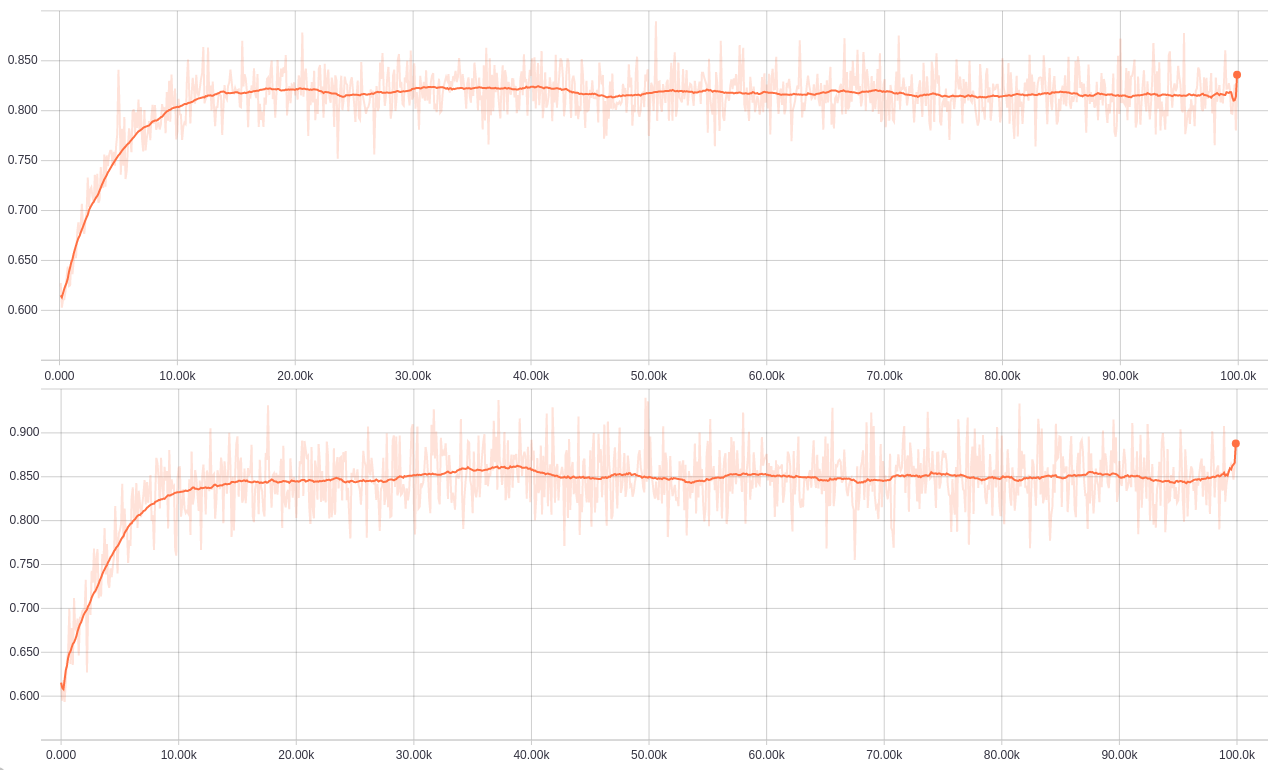
\includegraphics[width=\textwidth]{img/badanie_1.png}
  \end{figure}
\end{frame}
\begin{frame}{Badanie ze~zwiększoną liczbą iteracji}
    \begin{itemize}
        \item liczba iteracji: zwiększona do 144 tysięcy,
        \item cel: przeuczenie sieci.
    \end{itemize}
    \begin{table}[H]
        \centering
        \begin{tabular}{|l|l|l|l|l|l|}
            \hline
            \backslashbox{$\alpha$}{$\lambda$} & \cellcolor{orange!25}0.0005 & \cellcolor{orange!25}0.001 & 0.005 & 0.01 & 0.05 \\
            \hline
            0.00001 & 0.90 & 0.89 & 0.87 & 0.83 & 0.82 \\
            \hline
            0.00005 & 0.91 & 0.88 & 0.85 & 0.83 & 0.84 \\
            \hline
            0.0001  & 0.90 & 0.88 & 0.88 & 0.87 & 0.87 \\
            \hline
            \cellcolor{orange!25}0.0005  & 0.92 & 0.92 & 0.89 & 0.87 & 0.86 \\
            \hline
            0.001   & 0.89 & 0.87 & 0.87 & 0.83 & 0.83 \\
            \hline
        \end{tabular}
        \caption{Wpływ regularyzacji L2 ($\lambda$) i~normalizacji lokalnego kontrastu ($\alpha$) na~dokładność klasyfikacji
        sieci neuronowej przy~144~tysiącach iteracji. Czas badania: 64 godziny 17 minut i 23 sekundy}
        \label{table:wyniki2}
    \end{table}
\end{frame}
\begin{frame}{Dokładność sieci na zbiorze testowym i uczącym}
  \begin{figure}
    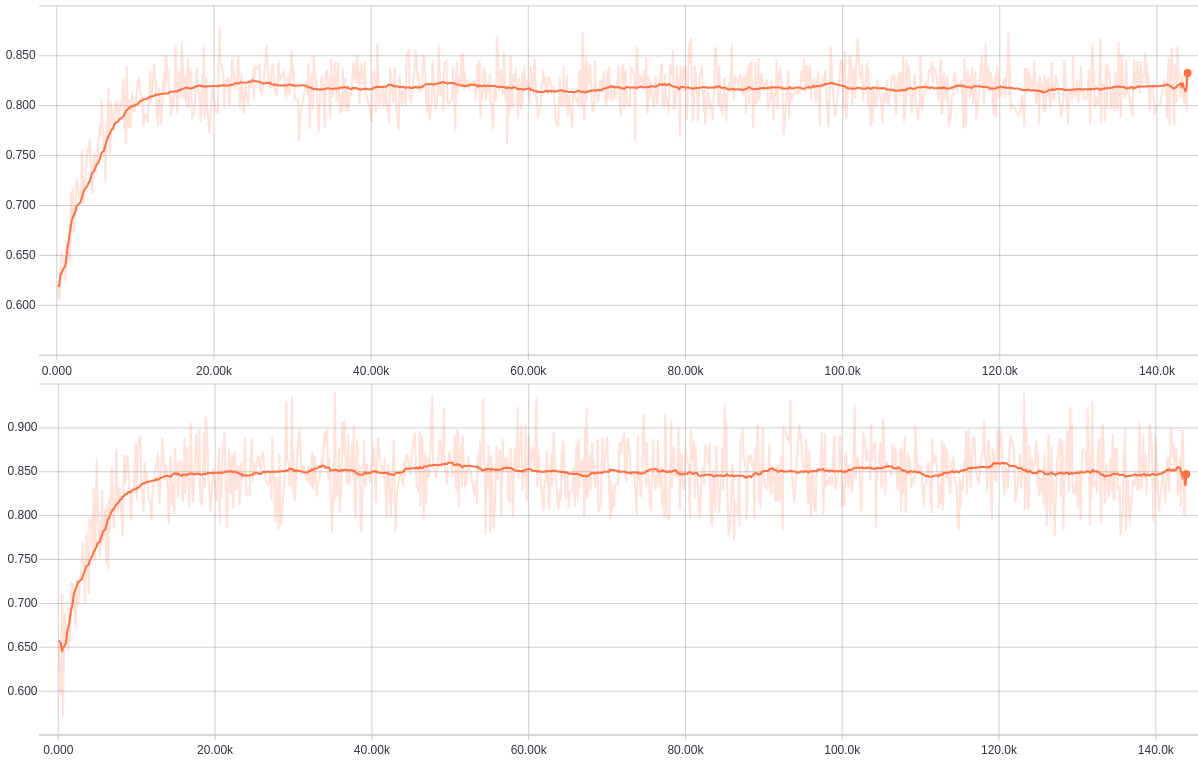
\includegraphics[width=\textwidth]{img/badanie_2.png}
  \end{figure}
\end{frame}
\begin{frame}{Ograniczony zbiór przykładów uczących}
    \begin{itemize}
        \item sześciokrotnie zmniejszono zbiór uczący,
        \item liczba iteracji: 144 tysiące.
    \end{itemize}
    \begin{table}[H]
        \centering
        \begin{tabular}{|l|l|l|l|l|l|}
            \hline
            \backslashbox{$\alpha$}{$\lambda$} & 0.0005 & \cellcolor{orange!25}0.001 & 0.005 & 0.01 & 0.05 \\
            \hline
            0.00001 & 0.76 & 0.80 & 0.74 & 0.69 & 0.69 \\
            \hline
            0.00005 & 0.78 & 0.77 & 0.72 & 0.69 & 0.67 \\
            \hline
            0.0001  & 0.77 & 0.78 & 0.79 & 0.74 & 0.73 \\
            \hline
            \cellcolor{orange!25}0.0005  & 0.78 & 0.82 & 0.76 & 0.76 & 0.72 \\
            \hline
            0.001   & 0.76 & 0.79 & 0.76 & 0.69 & 0.69 \\
            \hline
        \end{tabular}
        \caption{Wpływ regularyzacji L2 ($\lambda$) i~normalizacji lokalnego kontrastu ($\alpha$) na~dokładność klasyfikacji
        sieci neuronowej przy~sześciokrotnie mniejszym zbiorze uczącym. Czas badania: 62 godziny 43 minuty i 27 sekund}
        \label{table:wyniki3}
    \end{table}
\end{frame}
\begin{frame}{Dokładność sieci na zbiorze testowym i uczącym}
  \begin{figure}
    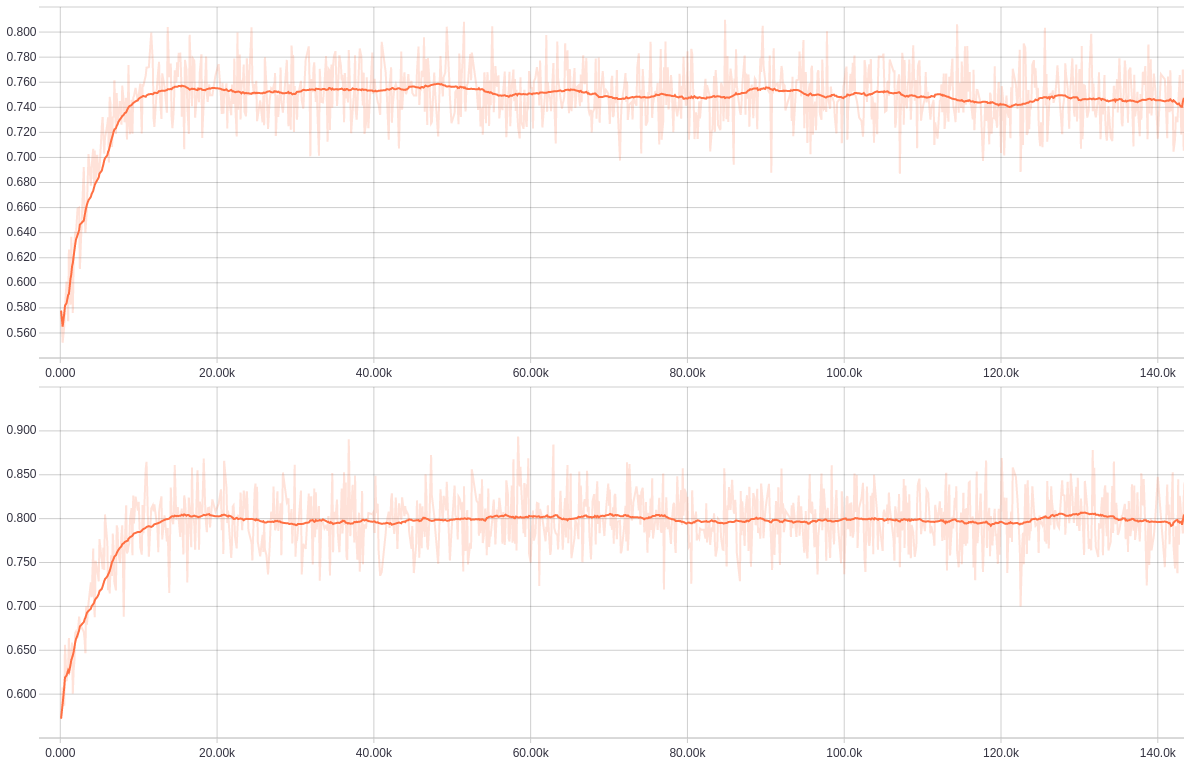
\includegraphics[width=\textwidth]{img/badanie_3.png}
  \end{figure}
\end{frame}
\begin{frame}{Badanie pomocnicze}
  \textbf{Cel:} Wyznaczenie pikseli najistotniejszych z~punktu widzenia klasyfikacji.
  \begin{figure}
    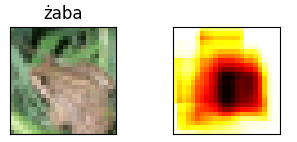
\includegraphics[width=\textwidth]{img/heatmap_1.png}
  \end{figure}
\end{frame}
\begin{frame}{Badanie pomocnicze c.d.}
  \begin{figure}
    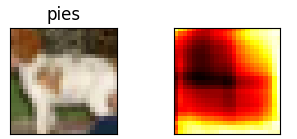
\includegraphics[width=\textwidth]{img/heatmap_2.png}
  \end{figure}
\end{frame}
\begin{frame}{Badanie pomocnicze c.d.}
  \begin{figure}
    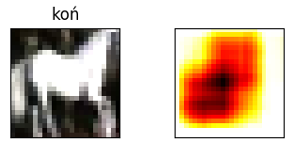
\includegraphics[width=\textwidth]{img/heatmap_3.png}
  \end{figure}
\end{frame}
\begin{frame}{Badanie pomocnicze c.d.}
  \begin{figure}
    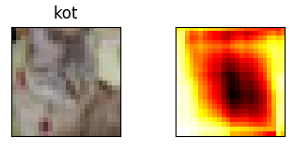
\includegraphics[width=\textwidth]{img/heatmap_4.png}
  \end{figure}
\end{frame}

\section{Podsumowanie}
\begin{frame}{Wnioski końcowe}
  Wnioski z badań:
  \begin{itemize}
    \item odpowiednio dobrane hiperparametry sieci mogą zapewnić lepszą jakość klasyfikacji,
    \item regularyzacja nie musi zwiększać jakości klasyfikacji,
    \item warto wykonywać badania pomagające zrozumieć, w jaki sposób sieć dokonuje klasyfikacji.
  \end{itemize}
\end{frame}
\begin{frame}{Bibliografia}
	\begin{itemize}
		\item Paweł Cichosz, ,,Systemy uczące się'', WNT Warszawa 2000,
		\item Steven Damelin, Willard Miller, ,,The Mathematics of Signal Processing'', CUP 2011
		\item Christian Theriault, ,,Extended coding and pooling in~the~HMAX model'', IEEE Xplore, 2013
		\item Andrew Y. Ng, ,,Feature selection, L1 vs. L2 regularization, and rotational invariance'', CoRR 2004,
		\item Yoshua Bengio, ,,Practical recommendations for~gradient-based training of~deep architectures'', CoRR 2012
		\item Matthew D. Zeiler, Rob Fergus, ,,Visualizing and Understanding Convolutional Networks'', CoRR 2013,
	\end{itemize}
\end{frame}

\begin{frame}{Pytania}
  \begin{figure}
    
\includegraphics[width=0.35\textwidth]{img/question-mark-red.png}
  \end{figure}
\end{frame}

\end{document}